\chapter{Thiết kế và đánh giá các pipeline học máy trong phát hiện mã độc}

\section{Tổng quan kiến trúc giải pháp}

\begin{figure}[h]
    \centering
    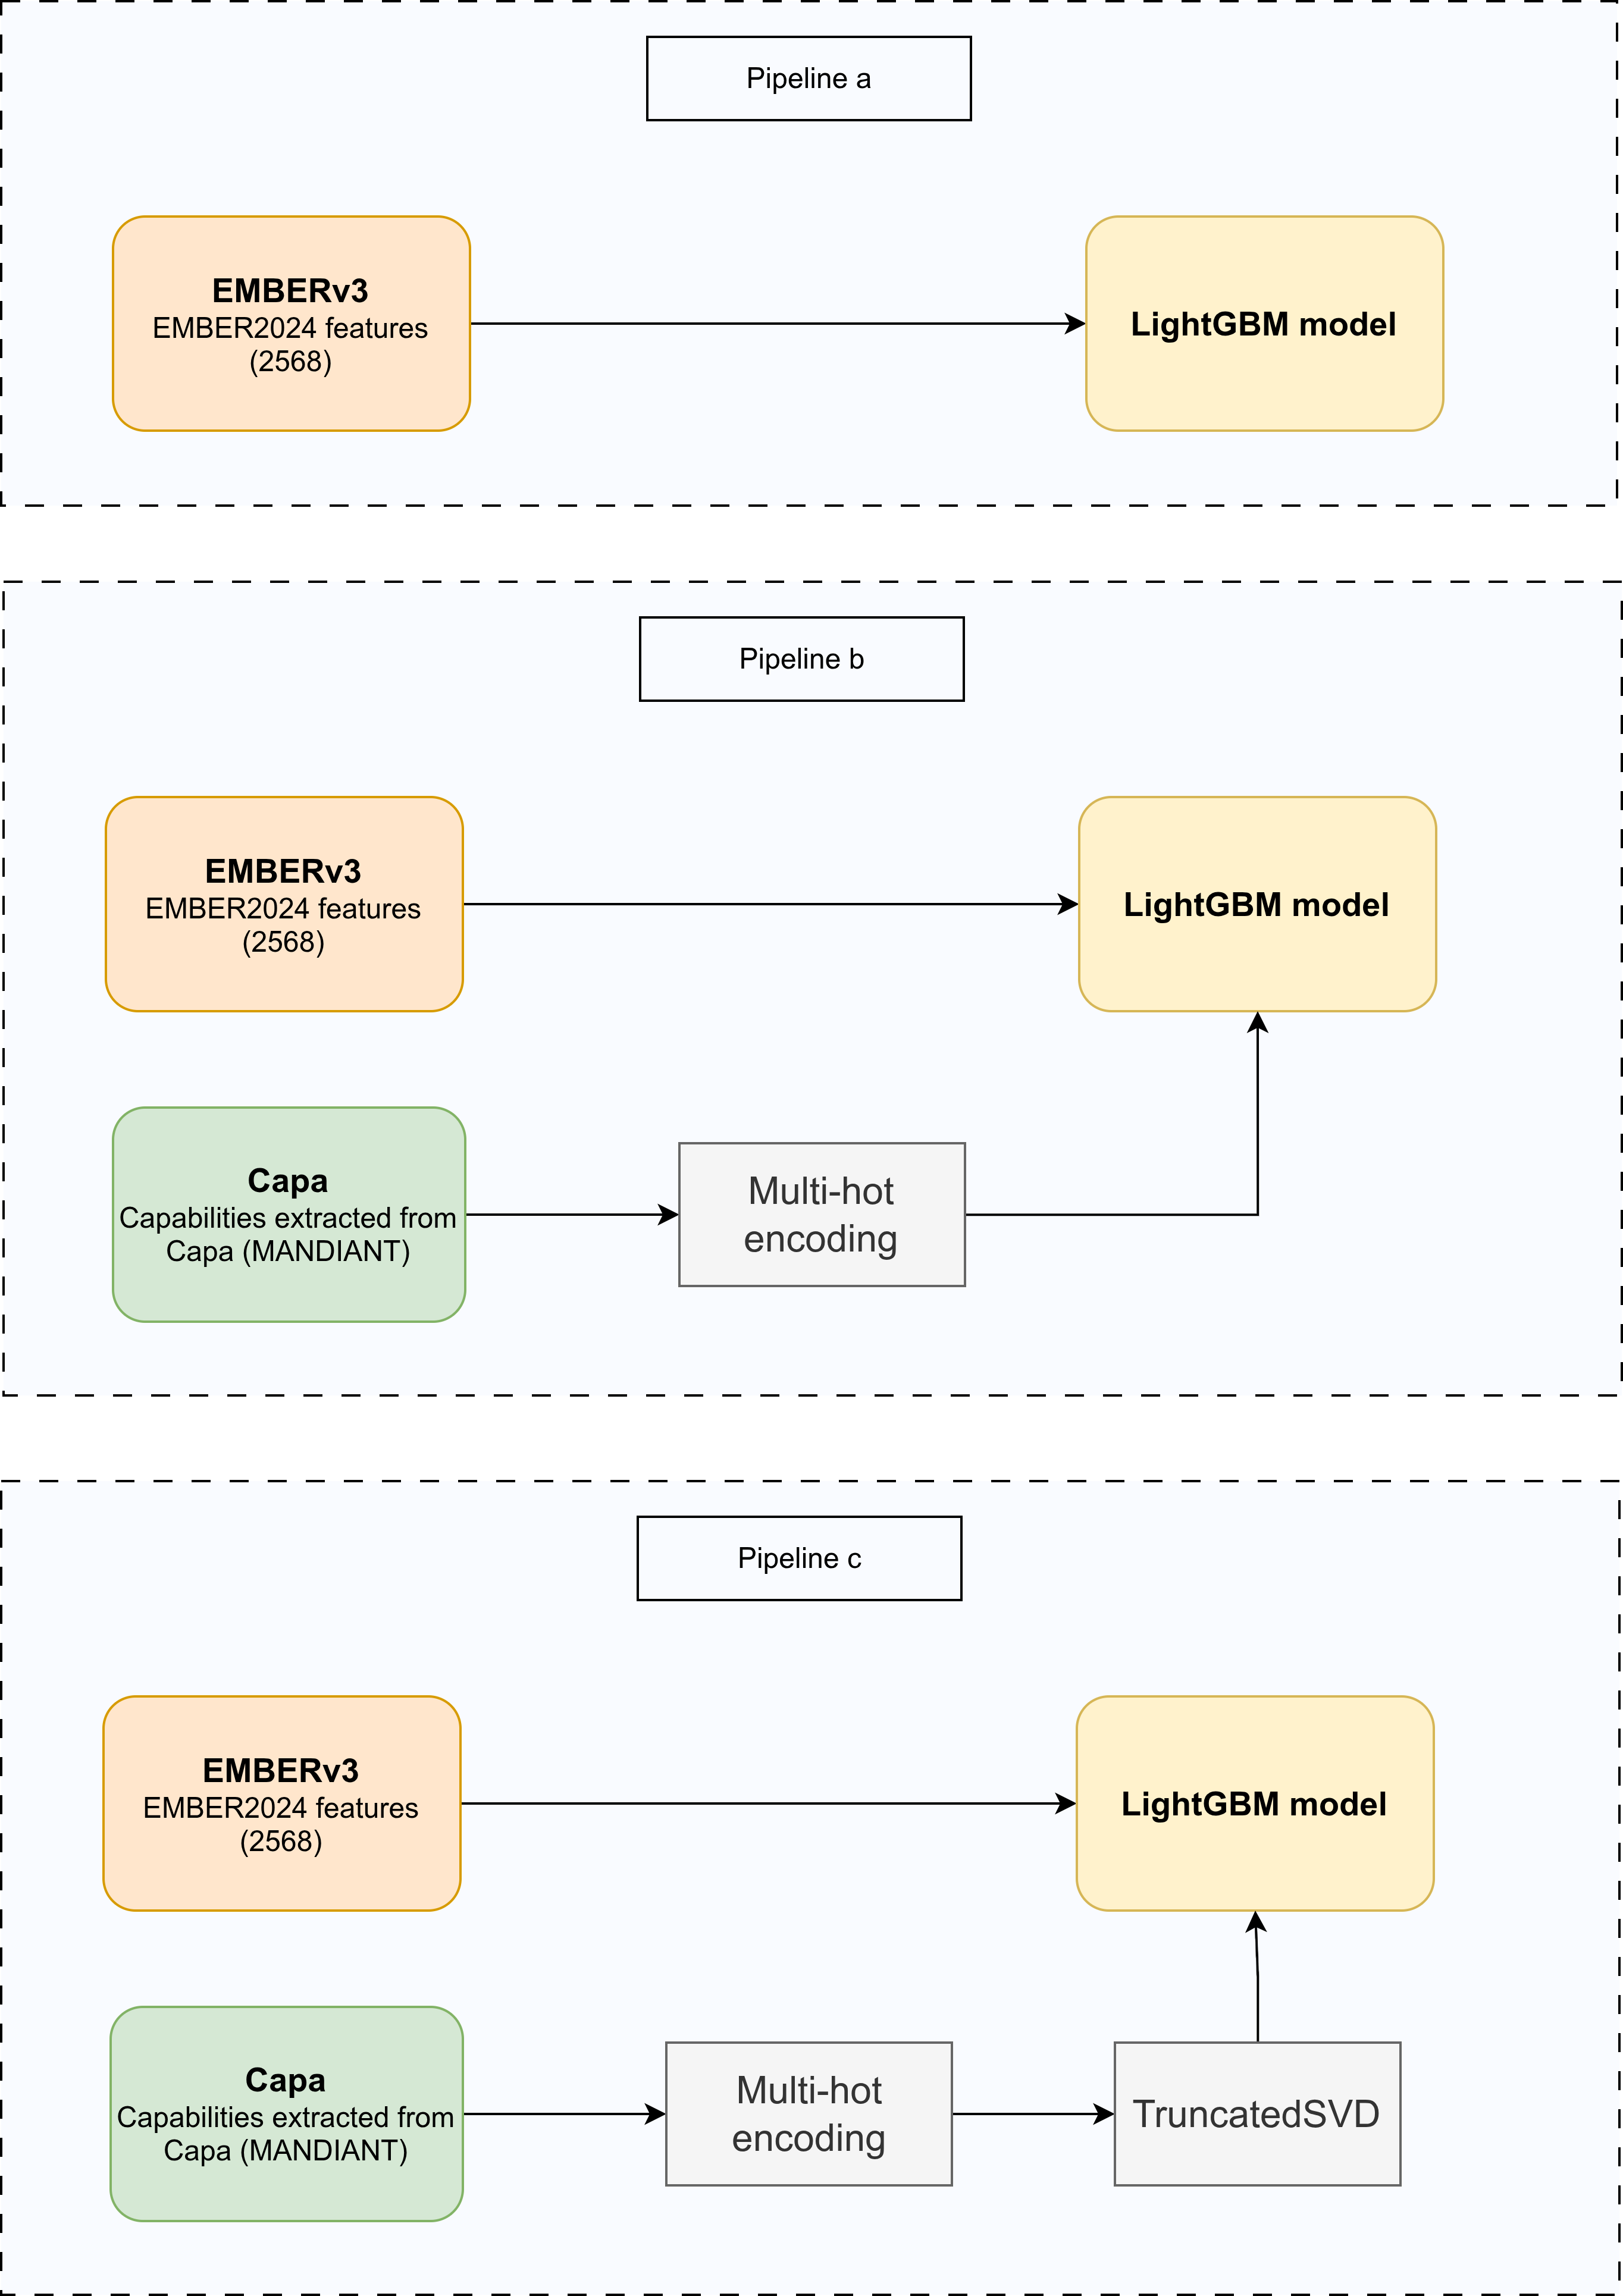
\includegraphics[width=\textwidth]{figures/ml-pipeline.png}
    \caption{Các pipeline học máy được sử dụng trong phát hiện mã độc PE.}
    \label{fig:pipeline_overview}
\end{figure}

Ở Chương~1, đề tài đã trình bày các nhóm đặc trưng tĩnh thường được
trích xuất từ file PE - bao gồm thông tin header, section, import
table, chuỗi văn bản và nội dung nhị phân - và cho thấy đây là nền
tảng hiệu quả để xây dựng mô hình phát hiện mã độc. Tuy nhiên, các
đặc trưng này chủ yếu phản ánh \textit{cấu trúc} của file PE, trong
khi thông tin về \textit{hành vi} và \textit{năng lực} tiềm ẩn của
mã độc - chẳng hạn khả năng mã hóa dữ liệu, leo thang đặc quyền hay
kết nối đến máy chủ điều khiển - vẫn chưa được khai thác. Chương
này đề xuất bổ sung loại thông tin trên thông qua kỹ thuật trích xuất
năng lực (capability extraction) bằng công cụ Capa, kết hợp với bộ
đặc trưng EMBER2024, đồng thời đánh giá liệu sự bổ sung này có giúp
cải thiện hiệu quả phân loại mã độc PE hay không.

Cụ thể, chương này xây dựng và so sánh \textbf{03 pipeline} học máy,
có sự khác biệt về cách xây dựng vector đặc trưng đầu vào, trong
khi giữ cố định mô hình (LightGBM), bộ siêu tham số (hyperparameters),
tập dữ liệu và chiến lược chia tập train/test
(Hình~\ref{fig:pipeline_overview}):

\begin{itemize}
    \item \textbf{Pipeline A}: chỉ sử dụng đặc trưng EMBER2024
        (baseline).
    \item \textbf{Pipeline B}: EMBER2024 kết hợp đặc trưng Capa dạng
        multi-hot encoding.
    \item \textbf{Pipeline C}: EMBER2024 kết hợp đặc trưng Capa sau
        khi giảm chiều bằng TruncatedSVD, thử nghiệm với các số chiều
        64, 128 và 256.
\end{itemize}

Với mỗi file PE đầu vào, pipeline luôn thực hiện bước trích xuất đặc
trưng EMBER2024 tạo ra vector 2.568 chiều. Tùy từng pipeline, có thể
triển khai bước trích xuất năng lực (capabilities) của các file PE
bằng Capa, chuyển đổi chúng thành vector bằng một phương pháp nhất định,
rồi ghép nối với vector EMBER2024 trước khi đưa vào LightGBM để phân
loại. Sự khác biệt giữa các pipeline nằm hoàn toàn
ở bước xây dựng vector đặc trưng, giúp cô lập và đo lường chính xác
đóng góp của từng nhóm đặc trưng.

Lựa chọn \textbf{LightGBM} làm mô hình phân loại xuất phát từ các
lý do đã trình bày ở Chương~1: hiệu năng cao trên dữ liệu đặc trưng
tĩnh nhiều chiều, tốc độ suy luận nhanh phù hợp với triển khai thực
tế, và khả năng diễn giải thông qua feature importance. Bản thân
LightGBM đã là một phương pháp ensemble nội tại (gradient boosting
của nhiều cây quyết định), do đó không cần thêm lớp ensemble bên
ngoài. Đáng chú ý, mô hình LightGBM pretrained do nhóm tác giả
EMBER2024 cung cấp - được huấn luyện trên toàn bộ tập dữ liệu gốc
- đạt ROC-AUC tổng thể là 0,9949, cho thấy tiềm năng của hướng
tiếp cận này khi được huấn luyện ở quy mô đầy đủ.













\section{Thiết kế các pipeline học máy}

\subsection{Tập dữ liệu EMBER2024}

EMBER2024 \cite{ember2024benchmark} là tập dữ liệu benchmark quy mô
lớn được thu thập từ tháng 9 năm 2023 đến tháng 12 năm 2024, bao gồm
hơn 3,2 triệu file thuộc sáu định dạng khác nhau (Win32, Win64, .NET,
APK, ELF và PDF). Vector đặc trưng sử dụng định dạng \textbf{EMBERv3}
với 2.568 chiều, là phiên bản mở rộng so với EMBERv2, bổ sung thêm
thông tin Rich header (dấu vết trình biên dịch), data directories,
và nhóm đặc trưng tổng hợp các cảnh báo phát sinh trong quá trình
phân tích file PE (PE file warnings). Các đặc trưng dạng danh mục hoặc chuỗi (tên
section, tên hàm import, chuỗi văn bản) được biểu diễn dưới dạng
vector hash kích thước cố định thông qua hashing trick (\texttt{FeatureHasher} của
\texttt{sklearn}), đảm bảo chiều dài vector nhất quán.

Trong phạm vi thực nghiệm so sánh các pipeline, do giới hạn tài nguyên
tính toán và thời gian chạy Capa, đề tài sử dụng một tập con gồm
\textbf{450.000 mẫu huấn luyện} và \textbf{50.000 mẫu kiểm tra},
được lấy mẫu từ tập dữ liệu gốc với tỷ lệ
malware/benign cân bằng và theo thứ tự thời gian: các mẫu cũ hơn
dùng để huấn luyện (train), các mẫu mới hơn dùng để kiểm tra (test).
Cách chia này mô phỏng sát
điều kiện triển khai thực tế, trong đó mô hình phải tổng quát hóa
sang các mẫu mã độc mới chưa từng xuất hiện trong dữ liệu huấn luyện.

Dưới đây trình bày chi tiết phương pháp triển khai của từng pipeline.

\subsection{Pipeline A: EMBER2024 thuần}

Pipeline A là baseline của thực nghiệm, sử dụng trực tiếp vector đặc
trưng EMBERv3 (2.568 chiều) làm đầu vào cho LightGBM mà không bổ sung
bất kỳ đặc trưng nào khác. Pipeline này phản ánh cách tiếp cận phổ
biến nhất trong các nghiên cứu sử dụng tập dữ liệu EMBER, đồng thời
là nền tảng để đánh giá mức độ đóng góp của đặc trưng Capa ở các
pipeline sau. Việc huấn luyện lại pipeline A trên cùng tập con 450K
mẫu - thay vì dùng mô hình pretrained gốc - nhằm đảm bảo việc so
sánh các pipeline là công bằng: tất cả đều xuất phát từ cùng một điều
kiện dữ liệu và cấu hình huấn luyện.

\subsection{Pipeline B: EMBER2024 kết hợp Capa multi-hot}

Pipeline B bổ sung đặc trưng năng lực (capability) từ Capa vào vector EMBER2024.
Với mỗi file PE, Capa trả về kết quả phân tích rất chi tiết;
song trong phạm vi đề tài, tác giả đã tiến hành cô đọng
kết quả phân tích trên về cấu trúc gồm ba thành phần:
danh sách \texttt{caps} (các
capability được nhận diện kèm namespace phân cấp), danh sách
\texttt{ttps} (chiến thuật và kỹ thuật theo MITRE ATT\&CK), và danh
sách \texttt{mbc} (hành vi theo Malware Behavior Catalog). Ví dụ, một
file PE sử dụng kỹ thuật packing có thể được Capa nhận diện với
capability \texttt{packed with upack} thuộc namespace
\texttt{anti-analysis/packer/upack}, ánh xạ sang tactic
\texttt{DEFENSE EVASION} trong ATT\&CK và behavior
\texttt{Software Packing} trong MBC. Quá trình
cô đọng này được gọi là \textit{remapping}.

\begin{lstlisting}[language=JavaScript, caption={Ví dụ output của Capa (remapped)}]
{
    "caps": [
        {
            "Capability": "reference analysis tools strings",
            "Namespace": "anti-analysis",
            "Addrs": []
        },
        {
            "Capability": "packed with upack",
            "Namespace": "anti-analysis/packer/upack",
            "Addrs": []
        },
        {
            "Capability": "contain an embedded PE file",
            "Namespace": "executable/subfile/pe",
            "Addrs": []
        },
        {
            "Capability": "contains PDB path",
            "Namespace": "executable/pe/pdb",
            "Addrs": []
        },
        {
            "Capability": "(internal) packer file limitation",
            "Namespace": "internal/limitation/static",
            "Addrs": []
        }
    ],
    "ttps": [
        {
            "Tactic": "DEFENSE EVASION",
            "Technique": "Obfuscated Files or Information :: Software Packing"
        }
    ],
    "mbc": [
        {
            "Objective": "DISCOVERY",
            "Behavior": "Analysis Tool Discovery :: Process detection"
        },
        {
            "Objective": "ANTI-STATIC ANALYSIS",
            "Behavior": "Software Packing"
        },
        {
            "Objective": "EXECUTION",
            "Behavior": "Install Additional Program"
        }
    ]
}
\end{lstlisting}

Trong pipeline B, tất cả các thành phần \texttt{caps},
\texttt{ttps} và \texttt{mbc} đều được sử dụng làm đặc
trưng, và được gọi chung (trong khuôn khổ khóa luận này)
là các capability. Từ điển capability toàn cục được xây dựng từ
tập huấn luyện gồm \textbf{1.250 capabilities} khác nhau.
Với mỗi file PE, danh sách capability được mã hóa thành
vector nhị phân dạng \textbf{multi-hot}:
mỗi chiều tương ứng với một capability trong từ điển, nhận giá trị 1
nếu file có capability đó và 0 nếu capability đó không hiện hữu
trong file. Vector Capa multi-hot (1.250 chiều) sau đó được
ghép nối với vector EMBER2024 (2.568 chiều) tạo
thành vector đầu vào tổng hợp 3.818 chiều cho LightGBM.

Nhược điểm của cách mã hóa này là vector Capa multi-hot
\textbf{rất thưa (sparse)}: với
nhiều file PE, chỉ một phần nhỏ trong 1.250
capability được kích hoạt, dẫn đến phần lớn các chiều nhận giá trị 0.
Điều này làm tăng chi phí tính toán và nguy cơ gây nhiễu cho mô hình.
Pipeline C được thiết kế để khắc phục hạn chế này.

\subsection{Pipeline C: EMBER2024 kết hợp Capa TruncatedSVD}

Pipeline C sử dụng lại vector Capa multi-hot của pipeline B,
sau đó áp dụng kỹ thuật giảm chiều \textbf{TruncatedSVD} lên
vector này trước khi ghép nối với vector EMBER2024 thuần
để đưa vào mô hình LightGBM. TruncatedSVD phân tích ma trận
đặc trưng Capa của toàn bộ tập huấn luyện, giữ lại $k$ giá
trị kỳ dị lớn nhất - tương ứng với các tổ
hợp capability có tính phân biệt cao nhất giữa các mẫu - và chiếu
xuống không gian $k$ chiều. Ma trận chiếu được fit trên
tập huấn luyện và áp dụng cố định lên tập kiểm tra, tránh data
leakage.

Để xác định số chiều nén (giảm) phù hợp, thực nghiệm được thực hiện với ba
giá trị: \textbf{64, 128 và 256 chiều}. Vector nén sau đó được ghép
nối với vector EMBER2024 2.568 chiều, tạo thành vector đầu vào tổng
hợp có số chiều lần lượt là 2.632, 2.696 và 2.824.

\subsubsection{Lý do lựa chọn kỹ thuật giảm chiều TruncatedSVD}

Vector Capa multi-hot là ma trận \textbf{rất thưa (sparse)}: với mỗi
file PE, chỉ một phần nhỏ trong 1.250 capability được kích hoạt, dẫn
đến phần lớn các chiều nhận giá trị 0. Đặc điểm này đặt ra yêu cầu
cụ thể đối với kỹ thuật giảm chiều: cần hoạt động hiệu quả trên dữ
liệu thưa và không làm mất đi ngữ nghĩa của giá trị 0.

PCA (Principal Component Analysis) là một trong các kỹ thuật giảm
chiều được sử dụng phổ biến nhất. PCA tìm các hướng có phương sai lớn
nhất trong dữ liệu bằng cách phân tích ma trận hiệp phương sai
$\mathbf{C} = \frac{1}{n}\mathbf{X}^\top\mathbf{X}$, trong đó
$\mathbf{X}$ là ma trận dữ liệu \textit{đã được mean-center} - tức
là đã trừ đi giá trị trung bình của từng chiều. Theo định nghĩa
thống kê chuẩn, mean-centering là bước cần thiết để PCA phân tích
đúng phương sai của dữ liệu. Tuy nhiên, với dữ liệu Capa multi-hot,
thao tác này gây ra hai vấn đề. Thứ nhất, mean-centering phá vỡ cấu trúc thưa: sau khi trừ giá trị
trung bình, các số 0 trở thành số âm và ma trận trở thành dense, làm
tăng đáng kể chi phí bộ nhớ và tính toán. Thứ hai, và quan trọng
hơn, giá trị 0 của một feature trong vector Capa multi-hot mang ý nghĩa xác định:
file PE \textit{không có} capability tương ứng với feature đó. Khi mean-centering biến các
số 0 thành số âm, PCA diễn giải sự \textit{vắng mặt} của một
capability như một tín hiệu âm có trọng số - trong khi đó chỉ là
trạng thái mặc định của nhiều file PE. Hệ quả là các thành phần
chính bị nhiễu bởi việc dịch chuyển này, thay vì phản ánh các tổ
hợp capability thực sự có tính phân biệt.

Để khắc phục hiện tượng trên, ta có thể bỏ qua bước mean-centering.
Tuy nhiên, cần lưu ý rằng về mặt toán học, khi áp dụng PCA, việc bỏ qua bước
mean-centering và chỉ giữ $k$ hướng có phương sai lớn nhất (tương ứng với
$k$ giá trị kỳ dị lớn nhất) chính là áp dụng TruncatedSVD.
Nói cách khác, nếu muốn dùng PCA mà tránh được vấn đề mean-centering
trên dữ liệu sparse như đã nêu, kết quả thu được chính là TruncatedSVD.
Do vậy, áp dụng TruncatedSVD trực tiếp là lựa chọn tự nhiên và đúng
mục đích sử dụng cho bài toán này.

\textbf{Cơ sở của TruncatedSVD.}
TruncatedSVD phân tích ma trận $\mathbf{X}$ thành tích:
\begin{equation}
    \mathbf{X} = \mathbf{U} \mathbf{\Sigma} \mathbf{V}^\top
\end{equation}
trong đó $\mathbf{\Sigma}$ là ma trận đường chéo chứa các giá trị kỳ
dị $\sigma_1 \geq \sigma_2 \geq \dots \geq 0$ sắp xếp giảm dần. Mỗi
$\sigma_i$ phản ánh mức độ phương sai mà thành phần thứ $i$ đóng góp
vào toàn bộ dữ liệu: $\sigma_i$ càng lớn thì thành phần đó càng mang
nhiều thông tin phân biệt giữa các mẫu. TruncatedSVD chỉ giữ lại $k$
giá trị kỳ dị lớn nhất, chiếu mỗi mẫu xuống không gian $k$ chiều
thông qua phép biến đổi $\tilde{\mathbf{x}} = \mathbf{x}\mathbf{V}_k$,
hoạt động trực tiếp trên ma trận $\mathbf{X}$ gốc mà không qua
mean-centering.

Ma trận $\mathbf{V}_k$ được fit trên tập huấn luyện và áp dụng cố
định lên tập kiểm tra, tránh data leakage. Kết quả là mỗi file PE
được biểu diễn bởi một vector $k$ chiều phản ánh các tổ hợp
capability có tính phân biệt cao nhất trong toàn bộ tập dữ liệu.

Như vậy, TruncatedSVD là lựa chọn phù hợp trong pipeline C, 
vừa đảm bảo hiệu quả tính toán trên
tập dữ liệu quy mô lớn, vừa tương thích tự nhiên với đặc trưng Capa
dạng thưa mà không làm mất đi tính chất thống kê quan trọng của dữ
liệu.

\subsection{Cấu hình huấn luyện}

Tất cả các pipeline đều sử dụng mô hình LightGBM với cùng bộ siêu
tham số, được lấy từ cấu hình gốc của dự án EMBER2024
\cite{ember2024benchmark}. Việc tái sử dụng cấu hình này có hai lý
do: nhóm tác giả EMBER2024 đã tối ưu bộ siêu tham số cho bài toán
phân loại mã độc PE trên tập dữ liệu này; và mục tiêu của thực nghiệm
là so sánh hiệu quả của các \textit{tổ hợp đặc trưng}, không phải
tối ưu siêu tham số - việc giữ cố định siêu tham số đảm bảo rằng
bất kỳ sự khác biệt nào quan sát được đều do đặc trưng đầu vào gây
ra. Một số thiết lập đáng chú ý bao gồm \texttt{num\_leaves = 64} và
\texttt{lambda\_l2 = 1.0} để kiểm soát độ phức tạp mô hình và tránh
overfit; \texttt{bagging\_fraction = 0.9} cùng
\texttt{feature\_fraction = 0.9} để tăng tính ngẫu nhiên trong quá
trình xây dựng cây; và \texttt{is\_unbalance = true} để xử lý mất
cân bằng nhãn nếu có.

Quá trình huấn luyện áp dụng cơ chế dừng sớm
\texttt{lgb.early\_stopping(50)}: dừng huấn luyện nếu điểm ROC-AUC
trên tập validation không cải thiện trong 50 vòng (rounds) liên tiếp.
Cơ chế này vừa ngăn overfit, vừa tiết kiệm thời gian huấn luyện khi
mô hình đã hội tụ. Số vòng tối đa là 500.





\section{Đánh giá và so sánh các pipeline}

\subsection{Lựa chọn độ đo đánh giá}

Trong bài toán phát hiện mã độc tại môi trường thực tế, False Positive
Rate (FPR) - tỷ lệ dương tính giả (tỷ lệ file lành tính bị phân loại nhầm thành mã độc)
- là chỉ số đặc biệt quan trọng. Một hệ thống cảnh báo nhầm quá
nhiều sẽ mất đi tính khả dụng và gây mất niềm tin của người dùng,
đặc biệt trong môi trường doanh nghiệp nơi hàng nghìn file được thực
thi mỗi ngày. Do đó, đề tài sử dụng \textbf{Partial AUC tại FPR
$\leq$ 0,5\%} làm độ đo chính - chỉ số này đo khả năng phát hiện
mã độc của mô hình trong vùng FPR cực thấp, phản ánh sát nhất yêu
cầu vận hành thực tế. \textbf{Full AUC} được sử dụng như độ đo phụ
để đánh giá hiệu quả tổng thể trên toàn bộ tất cả các ngưỡng phân loại.




\subsection{Kết quả thực nghiệm}

Bảng~\ref{tab:pipeline_results} trình bày ROC-AUC trên tập validation
theo các mốc iteration và kết quả cuối cùng trên tập kiểm tra của 05
cấu hình được thử nghiệm.

\begin{table}[h]
\centering
\caption{Kết quả so sánh các pipeline theo ROC-AUC (validation) và
AUC (test set).}
\label{tab:pipeline_results}
\resizebox{\textwidth}{!}{%
\begin{tabular}{lccccc}
\toprule
\textbf{Iteration} &
\textbf{Pipeline A} &
\textbf{Pipeline B} &
\textbf{Pipeline C} &
\textbf{Pipeline C} &
\textbf{Pipeline C} \\
& \textbf{(EMBER2024)} &
\textbf{(+Capa multi-hot)} &
\textbf{(+Capa SVD-64)} &
\textbf{(+Capa SVD-128)} &
\textbf{(+Capa SVD-256)} \\
\midrule
100 & 0.991358 & 0.991224 & 0.991288 & 0.991317 & 0.991116 \\
200 & 0.992569 & 0.992687 & 0.992706 & 0.992782 & 0.992563 \\
300 & 0.992794 & 0.993042 & 0.992997 & 0.993162 & 0.992987 \\
400 & ---$^{(1)}$ & 0.993130 & 0.993082 & 0.993283 & 0.993159 \\
500 & ---$^{(1)}$ & 0.993251 & 0.993194 & ---$^{(2)}$ & 0.993282 \\
\midrule
\multicolumn{6}{l}{\textit{Kết quả trên tập kiểm tra (test set)}} \\
\midrule
Partial AUC (FPR$\leq$0,5\%) &
0.8816 & 0.8843 & 0.8830 & 0.8838 & \textbf{0.8850} \\
Full AUC &
0.9922 & \textbf{0.9927} & \textbf{0.9927} & 0.9925 & 0.9926 \\
\bottomrule
\end{tabular}%
}
\vspace{4pt}
\begin{flushleft}
\small
$^{(1)}$ Dừng sớm (early stopping) tại iteration 251, ROC-AUC validation = 0.992813.\\
$^{(2)}$ Dừng sớm (early stopping) tại iteration 446, ROC-AUC validation = 0.993314.
\end{flushleft}
\end{table}

\subsection{Nhận xét kết quả}

Từ kết quả trong Bảng~\ref{tab:pipeline_results}, có thể rút ra một
số nhận xét sau:

\textbf{Đặc trưng Capa có đóng góp thực chất.}
Tất cả các pipeline có bổ sung đặc trưng Capa đều vượt baseline
pipeline A trên Partial AUC - độ đo chính của thực nghiệm. Điều
này cho thấy thông tin về năng lực mang lại giá trị phân biệt bổ sung
mà đặc trưng EMBER2024 thuần túy chưa phản ánh đủ. Đáng chú ý, ở
các iteration đầu (100--20 vòng), pipeline A và các pipeline Capa
có kết quả xấp xỉ nhau; sự khác biệt chỉ bộc lộ rõ từ iteration 200
trở đi, khi mô hình bắt đầu khai thác sâu hơn các mối quan hệ trong
đặc trưng.

\textbf{Pipeline A hội tụ sớm nhất.}
Baseline dừng sớm tại iteration 251, trong khi các pipeline có Capa
tiếp tục cải thiện đến iteration 400--500. Điều này phản ánh rằng
việc bổ sung đặc trưng Capa làm tăng độ phức tạp của không gian đặc
trưng, cho phép mô hình tiếp tục học thêm thông tin hữu ích trong
các vòng huấn luyện tiếp theo.

\textbf{TruncatedSVD-256 là lựa chọn tốt nhất trong nhóm pipeline C.}
Trong ba thử nghiệm giảm chiều bằng TruncatedSVD được thử nghiệm, SVD-256 đạt Partial AUC
cao nhất (0.8850) trên tập kiểm tra, vượt SVD-64 (0.8830) và SVD-128
(0.8838). Kết quả này cho thấy việc giữ lại nhiều chiều hơn giúp bảo
toàn thông tin năng lực tốt hơn, đặc biệt trong vùng FPR thấp.
SVD-128 dừng sớm nhất trong nhóm (iteration 446) và đạt Full AUC
validation cao nhất (0.993314), nhưng lại không dẫn đến Partial AUC
tốt nhất trên tập kiểm tra - điều này gợi ý rằng hội tụ nhanh
không đồng nghĩa với hiệu năng tốt trong vùng FPR thấp.

\textbf{So sánh pipeline B và pipeline C.}
Pipeline B (Capa multi-hot) đạt Full AUC bằng với SVD-64 (0.9927),
nhưng Partial AUC (0.8843) thấp hơn SVD-256 (0.8850). Điều này cho
thấy TruncatedSVD không chỉ giúp giảm chi phí tính toán mà còn có
tác dụng lọc nhiễu, loại bỏ các chiều capability ít có tính phân biệt
và giữ lại các tổ hợp capability quan trọng nhất.

\subsection{Thảo luận và lựa chọn pipeline triển khai}

Dựa trên kết quả thực nghiệm, đề tài lựa chọn hai pipeline để đưa
vào triển khai tại Chương~3, với tiêu chí cân bằng giữa hiệu quả
phát hiện và yêu cầu vận hành:

\textbf{Pipeline A} được lựa chọn cho \textbf{dịch vụ antivirus
offline tại endpoint}. Mặc dù Partial AUC thấp hơn các pipeline có
Capa, pipeline A có ưu thế quyết định về tốc độ: trích xuất đặc trưng
EMBER2024 thuần túy có thể thực hiện trong dưới một phân mười giây đối
với file nhỏ, phù hợp với yêu cầu phân tích thời gian thực tại máy endpoint.
Hơn nữa, khi triển khai tại endpoint, đề tài sử dụng mô hình
LightGBM gốc được nhóm tác giả EMBER2024 cung cấp - đã được huấn
luyện trên toàn bộ 2,6 triệu mẫu - thay vì mô hình huấn luyện trên
tập con 450K mẫu, nhờ đó đảm bảo hiệu năng phân loại tốt nhất có thể
cho dịch vụ offline.

\textbf{Pipeline C (SVD-256)} được lựa chọn cho \textbf{dịch vụ phân
tích sâu online (deep-analysis-server)}. Trong ngữ cảnh này, thời gian
phân tích có thể kéo dài hơn do người dùng chủ động yêu cầu phân tích
một file cụ thể, và kết quả trả về cần mang nhiều thông tin ngữ nghĩa
hơn - bao gồm danh sách capability được trích xuất và giải thích
SHAP. Bên cạnh đó, pipeline C cũng đạt Partial AUC cao nhất (0.8850) trong số các
pipeline được thử nghiệm.
